\newcommand{\gae}[0]{Google App Engine}
\newcommand{\mr}[0]{\emph{MapReduce}}
\chapter{Google App Engine}

\section{Description}
\gae{} is both a platform and infrastructure as a service cloud computing environment provided by Google. This platform allows developers to develop and deploy distributed web applications on Google's infrastructure, abstracting all notion of parallelism away from the developer. Google takes care of all the parallelism behind the scenes while guaranteeing a fast, scalable environment for developers to work in. 
%cite PaaS http://arxiv.org/pdf/0907.4622.pdf

While Google is secretive about the underlying architecture of its servers, \gae{} is most likely deployed across Google's servers using some variation of \mr{}. Developed in the late 1990s, \mr{} is a method for distributing programming tasks across multiple processes. MapReduce is based on functional programming paradigms, specifically the \emph{Map} and \emph{Reduce} functions typically found in such languages. Developers supply a list of data, and a function to apply to that data. This is the \emph{Map} step in \mr{}. Another function is also provided by the developer, to be used in the \emph{Reduce} step, which combines the resulting list of data to obtain the final result. All parallelism is handled by \mr{}, abstracting all notion of parallel programming away from application development. This is \mr{}'s strength and what allows Google to provide guaranteed automatic scaling to users of \gae{}.

% Map Reduce Scheduling: (Can be used in final report for comparison)
%
% 	- Highly fault tolerant. When Jobs fail, reassigns to another idle node.
%	- atomic commits
%	- Straggler nodes
%		- When MapReduce near completion, schedules backup executions of final in-progress job(s). Completes whenever primary or backup completes
%		- takes 44\% longer to complete when disabled.
%	- Combiner function can be specified that does partial merging on worker nodes before being sent to the network

\begin{center}
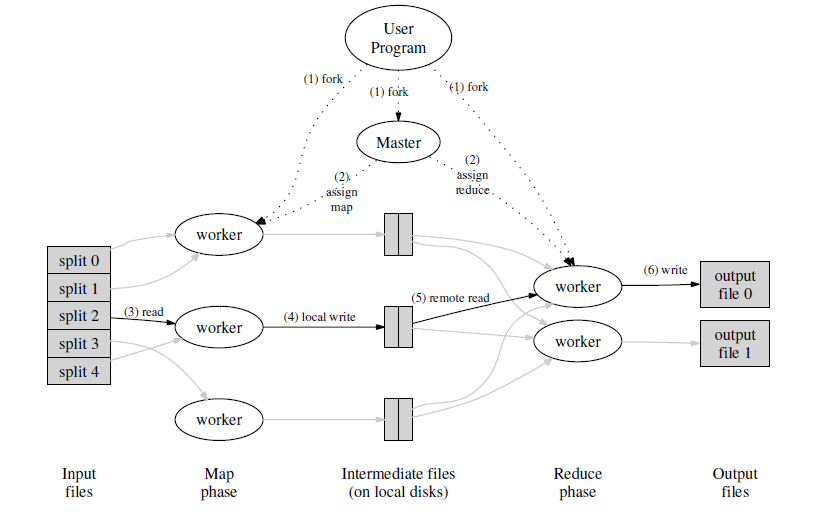
\includegraphics[scale=0.4]{figs/MapReduce.png} \\
\texttt{Overview of MapReduce execution} % Citation %
\end{center}

\section{Application Runtime Environment}
\gae{} provides three runtime environments to develop and deploy applications in; Python (2.5.2 and 2.7.2), Java (SDK 5 or 6), and Google's own language, Go (experimental). Developers can also use other JVM based languages such as Ruby and JavaScript in the Java runtime environment. A local development environment which emulates \gae{} is also provided. 

These are not the standard runtime environments typically used for development in these languages. Google provides a restricted version of the respective standard libraries, allowing google to effectively scale and sandbox the runtime environments. The restrictions to the standard libraries are as follows:
\begin{itemize}
\item Computers can only connect to \gae{} over HTTP(S) on standard ports.
\item No filesystem access.
\item Applications can only access other computers using Google's provided web services.
\item Code can only run in response to a web request, queued task or scheduled task. 
\item Applications must take no longer than 60 seconds to respond to a request.
\end{itemize}

In addition to this restricted standard library, Google also provides a number of services:
\begin{itemize}
\item APIs for authenticating users through Google Accounts.
\item An admin console for mantaining existing applications
\item Image manipulation
\end{itemize}

\section{Data Storage}
While Google restricts the standard libraries of its runtime environments to prevent reading and writing to file, two main methods are provided for persisent concurrent data storage; Memcache and the Datastore.

\subsection{Memcache}
Memcache is a service provided by Google which provides a high performance, in memory key-value store. This is stored in cache and can be accessed across multiple instances of an application.

\subsection{Datastore}
One of \gae{}'s features is its automatically scaling datastore, a database-like system which allows for persistent storage within an application. The Datastore is a NoSQL schemaless object datastore, allowing for persistent storage of Objects. 

Objects in the datastore are entities with a \emph{kind} and a set of a properties. Using Java as an example, objects can be persistently stored in the datastore; the class is the entity's \emph{kind} and its properties are the object's attributes. These can be stored and accessed using either JDO or JPA's persistence managers and query engines.

The Datastore is based on the \emph{High Replication Datastore} design: a system based on the \emph{Paxos algorithm} is used to replicated data across multiple servers. The datastore is strongly consistent and uses optimistic concurrency control. This means that transactions can proceed without locking because it assumes that multiple transactions can be completed without affecting each other. When a commit is made to the datastore each transaction checks that no others have modified the relevant part of the datastore since the transaction started. If changes are found, the commiting transaction is rolled back.
 
\subsection{External Services}
While the datastore is automatically scalable and provides high performance, it does not guarantee, and in some cases allow for atomic transactions where relations between objects exist. Some situations require relational algebra, so Google also provides access to its relational SQL database service known as \emph{Cloud SQL} from within \gae{}. 

Google also provides access to its \emph{Cloud Storage} system, which allows for storage of files up to a terabyte in size. This however cannot be accessed from the Google Go runtime environment.

\section{Cost}
\gae{} can be used for free, giving any developer 1 GB of storage and up to 5 million page views a month. Once either of these limits are exceeded service to an application will be cut off for that month unless billing options are implemented. Pricing for \gae{}'s services is complex, containing varying costs for reads/writes to the datastore and hours per instance required. These can be found at \emph{https://developers.google.com/appengine/docs/billing}. A minimum of \$2.10 per week must be spent if the billable services are used, and developers can specify a maximum daily budget.
